\documentclass[normalsize]{acm_proc_article-sp}
\usepackage[english]{babel}
\usepackage{natbib}
\usepackage{url}
\usepackage[colorlinks,linkcolor=black,citecolor=black,urlcolor=blue]{hyperref}
\newcommand{\abc}{Securety Group Name}
\usepackage{listings}
	\lstset{
		%alsoletter={Securety Group Name},		
		%morekeywords={S, Security Group Length, Securety Group Name},
		%keywordstyle=\bfseries\color{red},
		basicstyle=\ttfamily\tiny,
		tabsize=5}
	
\makeatletter
\AtBeginDocument{
	\renewcommand{\thefigure}{\arabic{section}.\arabic{figure}}
	\@addtoreset{figure}{section}
	\renewcommand{\thetable}{\arabic{section}.\arabic{table}}
	\@addtoreset{table}{section}
	\@addtoreset{footnote}{section}}
\makeatother

\begin{document}
%Titlepage
\title{Secure service discovery in open networks with SLP}
\numberofauthors{2}
\author{
Markus Alexander Kuppe - \email{8kuppe@informatik.uni-hamburg.de}\\
Vitali Amann - \email{5amann@informatik.uni-hamburg.de}\\\\
University of Hamburg\\
\today
}

\maketitle

\begin{abstract}
Mobile Ad-Hoc and open networks become increasingly common due to the wide availability of mobile device technology. When such devices enter a network, they want to learn about services offered by other peers or advertise own services. Service discovery protocols have been around to answer this requirement for years. A most prominent and widely adopted one is Service Location Protocol (SLP). However, SLP has not been designed for open networks, but for trustworhty and reliable networks. Thus the protocol has to undergo a renewal to make it fit for open networks.\\
This paper focuses on the security implications that arise from SLP's usage in open networks and gives a detailed threat analysis. Afterwards security extensions are proposed to address the identified shortcomings.
\end{abstract}
\keywords{Ad-hoc networks, open network, service discovery, service location protocol, security, trust, pki, web of trust, multicast, secure SLP}

%Chapter 1: Introduction
\section{Service discovery basics}\label{sec:intro}
Recent advances in computer science make it possible to build small mobile devices with many features. They have a long battery lifetime, a powerful processor unit and can handle more and more advanced applications. Mobile devices are here not just Notebooks but also PDAs, mobile phones, MP3 Players and so on. Due to the growing abilities of mobile devices it became reasonable to connect them. The idea is to connect several mobile devices to a network to allow them to communicate with each other and to share their services. In this paper we want to observe the possibilities offered by service discovery protocol (SLP). We will compare its current weaknesses and create suggestions how to fix them. To begin with, we first introduce the usage of such mobile devices in an open network.\\
A possible scenario is for example a hotel where we can find several user groups. For hotel employees it would be useful if special hotel services would be multicast. Those services can be like ``available rooms", ``technical control", ``room cleaning" and so on. In this way a hotel employee has a possibility to be mobile and still make his work and controlling several hotel properties. Another user group could be the guests. For this group there are other useful services like ``room service", ``environment map", ``weather", ``great attractions" and so on. A guest would have a possibility to order something to his/her location (not necessarily into the room) or easily find out some interesting attractions near the hotel. But as both groups are in same network, there is also a need to hide and/or secure some services from unauthorized users. In case a vicious person gets access to the employee services he could control technical features or checking other guests in/out. Those problems should be prevented early. The guests shouldn't even be able to see the services for hotel employees and neither should they be able to use them. To hide the services and encrypt communication is already a way to prevent attacks on those services (more details will be discuss in section 3).\\
Other possible scenario is for example a person with a mobile phone who offers phone calls over an open network (we assume such a person has a national flat rate). Another person with a notebook could use such a service to call someone. Possible attackers could track the user and get the phone number he is calling or an attacker could betray the service provider with an international phone call. In this case it is reasonable to encrypt the communication between service provider and user and there should be a kind of trust that the service user doesn't use the service in a wrong way. But to make such an infrastructures work in this way there are some requirements to fulfill: 
\begin{itemize}
\item server and client have to be on the same network 
\item both should speak the same lingo (use same protocols for example) 
\item to use or provide sensitive services they need some kind of security to find services in the network 
\end{itemize}
The main subject of this paper is service discovery and its security issues that arise in hostile environment like open networks. This paper separates the service discovery and service invocation from each other and we don't discuss security issues after service invocation here. However, to understand the service discovery security and their weaknesses we first need to understand the basics of service providing and service discovery.\\

\subsection{Open network}
In this paper we are talking about networks as free or open networks. An open network is a network for everyone even for bad guys. It provides the possibility that everyone who wants to join this network will join it. In this way the network allows the communication between every peer that is a part of this network. Also the idea of an open network is to create a network everywhere without complicated operations. So the open network is very dynamical. The network can be created centralized with servers or it can be created decentralized with peer to peer communication. All peers can connect or disconnect to the network anytime and without any restrictions. In this way there are no constrains and you can connect every possible devices with each other like personal computers, servers, notebooks but also printers, mobile phones, mp3 players and other portable or stationary devices. Open networks aren't necessarily based on IPs but in this paper we work with service location protocol (SLP) so we presume the communication is IP based. How the open network works is not a part of this paper. Furthermore we don't treat security issues in open network itself and assume that it is secure \citep{Foundation2009}.

\subsection{Service discovery architecture}
There are three important architecture approaches used for service
discovery \citep{Ververidis2008}.

\subsubsection{Directory-based architecture}
In directory-based architecture network peers have three possibilities how they can act. A network peer can offer its services as SA (\textbf{s}ervice \textbf{a}gent) to other peers, it can use discovered services as UA (\textbf{u}ser \textbf{a}gent) and a network peer can act as DA (\textbf{d}irectory \textbf{a}gent) which caches services provided by other SAs and forwards them to user agents. Because an open network is a dynamic network it can't be assume that there is always a reachable directory agent. But it is also possible that more than just one DA is operating in an open network. A directory agent is an important instance in this architecture and is essential to keep the network alive. All devices (service agents) which want to provide their services have to register them by a directory agent.
They register their services by sending service description (e.g. service name, server IP, description what the service can do, etc.) to the directory agent which stores all that information. As soon as a user agent wants to use a service, it sends via unicast a request for a searched service to the DA or it request all services which the DA stores. After receiving the information about the requested service the UA can connect to the SA (also see figure 1.1). This architecture reduces the entire communication in the network. The devices don't need to communicate via multicast anymore, hence they don't force their resources which mean they also save battery lifetime. But on the other hand the benefit of this architecture is their biggest handicap at the same time. The DA in some kind centralizes the network and makes it vulnerable. If a DA leaves the network, the network also loses all the services that DA had stored. First problem arises for the SAs and UAs that they need a technique to notice a missing DA. And the other problem is that service providers and users have to find a new DA and for this time their services aren't reachable. In the worst-case they don't find a new DA and indirectly get excluded from the network. There are some approaches to avoid such cases but they aren't part of this paper so we won't discuss them here.

\begin{figure}[h]
\centering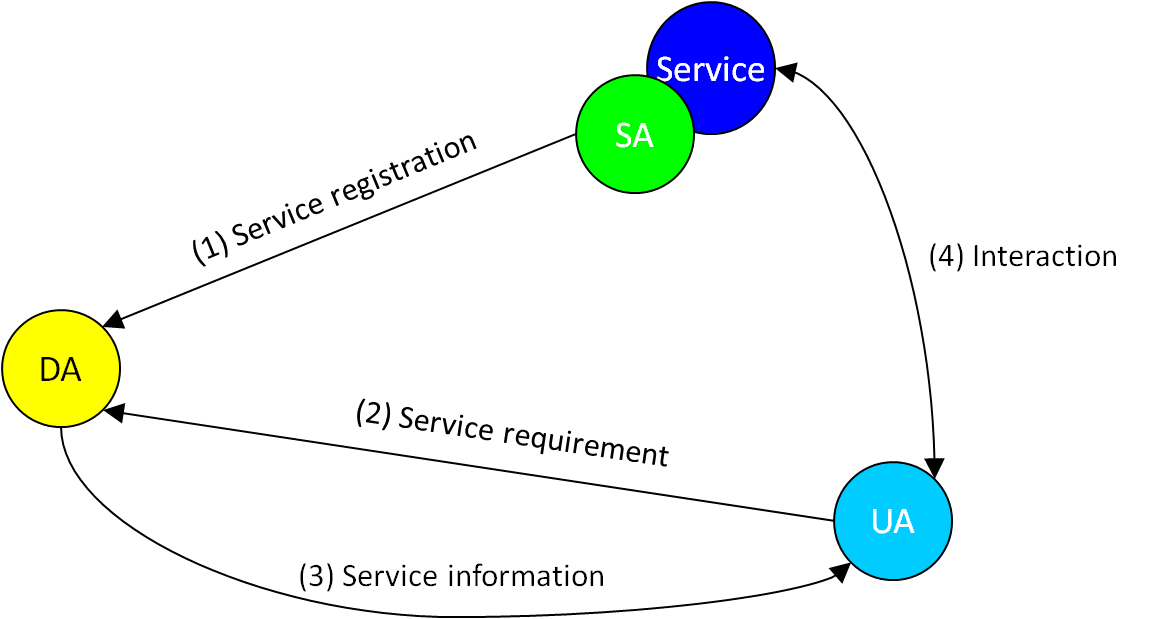
\includegraphics[width=0.5\textwidth]{Images/directory-based_architecture}
\caption{Directory-based architecture}
\end{figure}\noindent

\subsubsection{Directory-less architecture}
The directory-less architecture is quite contrary to the directory-based architecture. In this architecture the network peers can just act as service agents and as user agents. There is no directory agent so the service discovery should perform in other way. There are several approaches how this can be done. Service agents can distribute their services via multicast periodically send to the network. If a UA is interested in an offered service it requires the service information from the SA (also see figure 1.2). User agent can also discover services on their own by sending periodically a defined service request via multicast to the network till it gets an answer from a SA. Or a user agent can send a request to some network peers in its scope. In case a peer offers such a service it replies to the user agent otherwise the peer forwards the request to its neighbors and so on. In this architecture there is no central instance and it provides a much more stable network structure. However the communications via multicast drain more computation and battery lifetime from each network peer. Also to discover a service can take much longer compared to the directory-based architecture because there is no central authority that provides all services with their information.

\begin{figure}[h]
\centering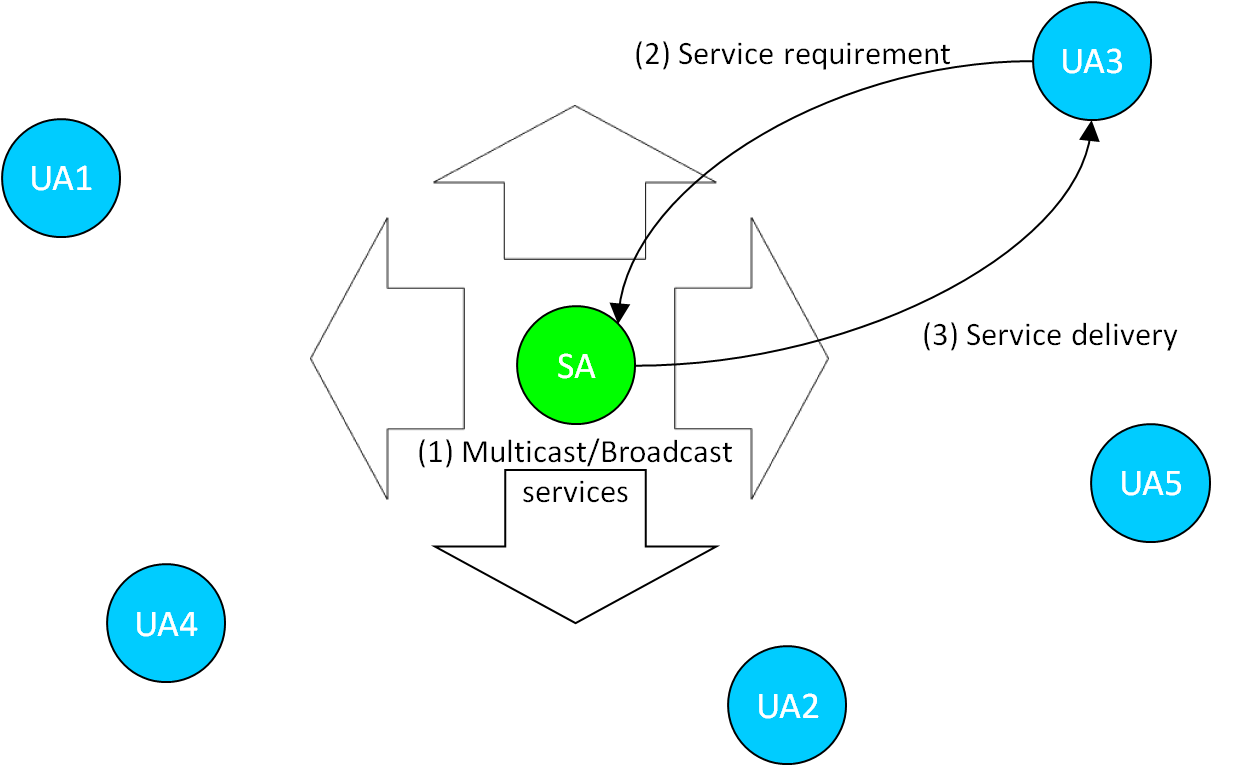
\includegraphics[width=0.5\textwidth]{Images/directory-less_architecture}
\caption{Directory-less architecture}
\end{figure}\noindent

\subsubsection{Hybrid architecture}
Hybrid architecture is a compromise of directory-based and directory-less architecture. Hybrid architecture combines the benefits of both other architectures. Like in directory-based architecture there are also three possibilities how a network peer can act (SA, UA and DA). To provide services a service agent first searches for a directory agent. In case a directory agent was found the service agent acts like in directory-based architecture and sends its service information to the DA and the DA is used by user agents to discover the services. In other case where no DA was located or all DAs left the network the SA acts like in directory-less architecture and periodically broadcast its services to the whole network. This architecture uses the benefits of the directory-based architecture to provide and discover services efficiently and to spare too many broad- and multicast communications in the network to keep battery lifetime from each network peer longer alive. At the same time the architecture offers a solution for the worst-case where no DAs are available in the network so the network won't die. The service location protocol, we will discuss below, is also based on the hybrid architecture.

\subsection{Secure service discovery basics}
Section 1.2 introduced some solutions how services can be provided and discovered in an open network. But there are also some security issues that prevent a secure usage of such a network. To safety use service discovery we have to fulfill at least the traditional security requirements:

\begin{itemize}
\item Authentication 
\item Authorization 
\item Integrity 
\item Confidentiality 
\end{itemize}
\citet{Cotroneo2004} suggests securing the registration and deregistration of the services. If a service is to be registered/deregistered it is important that authentication, authorization, integrity and confidentiality are maintained. In that way only authorized service agents can register or deregister their services. While registering a service, the communication has to be secured (by encryption) to prevent changes in the transferred information (integrity and confidentiality). With these common techniques many attacks like replay attack, user tracking or manipulating service information can already be prevented or become at least difficult (see also following sections). But just to secure the registration and deregistration is not enough. After the service discovery phase a user agent and service agent need an authentication between each other to keep their trust. Only authorized network peers should access the registered services. Authentication is needed in first way for the service agent who gets the information that the service was delivered to the right node if authentication was successful. And if a service agent authenticates itself by the user agent, user agent can be sure to trust the delivered service. Specific techniques to solve this problem are for example ``Web of Trust" and ``Public Key Infrastructure" which will be discussed in section 3.1.\\
Another important feature is the availability. It is not a secure issue in a first way but a network should also be able to detect broken service providers and delete them from the services list to prevent possible exploitations.

%Chapter 2: SLP Overview
\section{Service Location Protocol}\label{sec:slp-overview}
The Service Location Protocol (SLP) is an IETF standard published in 1997. It has been superseded by version 2 \citep{Guttman1999} in 1999. Since its publication, it has seen wide adoption ranging from embedded devices up to enterprise scale applications. This paper will be based on SLPv2, though most of it possibly also applies to SLPv1.

\subsection{Protocols basics\label{sub:Protocols-basics}}
SLP is a discovery-only protocol which explicitly leaves the service invocation out. A service is represented by a service description that consists of a Uniform Resource Locator (URL) \citep{Berners-Lee1994} which uniquely locates the service in a network. Additionally a service description may contain attribute-value pairs.\\
A UA may query for services by optionally using a Lightweight Directory Access Protocol (LDAP) \citep{Howes1997} style filter. A query is sent out via multicast \citep{Armstrong1992} and answered by all matching SAs. This mode is called multicast convergence. If present, a DA acts as a service cache. In this mode, UAs as well as SAs are required to not communicate over multicast directly, but via the DA employing unicast communication. Messages are sent via User Datagram Protocol (UDP) as long as they do not exceed the Maximum Transmission Unit (MTU). In case of the latter Transmission Control Protocol (TCP) has to be used.\\
SLP requires SAs to register with it when a DA enters the network. Making SAs aware of newly available DAs is done by sending out multicast beacons by the DA. These messages are called DAAdvertisements.\\
SLP allows grouping services in scopes. A scope is a string that is part of all messages\footnote{Except service Request of type ``service:directory-agent" and ``service:service-agent"}. SAs and DAs may only answer to queries if configured for the given scope. If no scope is provided, the default scope is automatically applied. SLP specifies no means to learn of all existing scopes, which might lead to regard scoping as a security feature. However, since communication is unencrypted, a simple traffic sniffer allows an attacker to learn of all existing scopes.

\subsection{Authentication and Integrity\label{sub:Authentication-and-Integrity}}
Regarding security, SLP provides only pre-established trust relationships based on digital signatures using asymmetric keying. This allows DAs, SAs and UAs to authenticate each other.\\
On top of this, asymmetric keying allows to verify message integrity by all parties. Though selected parts of the message only are included in the signature.\\
The trust relationship between SLP agents is established by the network administrator who supplies the agents with the correct public and private keys. A key distribution protocol is not part of SLP.\\
Authentication is used during service registration and registration cancellation. The same signature is needed to cancel a service registration, which has been used to register the service description initially. Incremental service registrations are an optional feature in SLP that allows an SA to incrementally update a service description. RFC 2608 leaves out if incremental service registrations are required to come from the same signature.\\
The built-in algorithm is Digital Signature Algorithm (DSA) \citep{Kravitz1993} with Secure Hash Algorithm 1 (SHA1) \citep{Eastlake3rd2001} used for hashing, though other algorithms are possible as vendor extensions.

\subsection{Replay Prevention\label{sub:Replay-Prevention}}
``A replay attack is a form of network attack in which a valid data transmission
is maliciously or fraudulently repeated or delayed" \citep{Wikipedia2009}. To
prevent such replay attacks, SLP timestamps each signed message with a 32-bit
unsigned fixed-point number UNIX time. The time stamp indicates when the
signature expires. Using a time stamp does not fully prevent replay attacks as it leaves
a door open to attacks for the duration of the signature life-time. Hence a
nonce\footnote{Random, non-guessable and externally non-influenceable data} that
is to be included in the initial request (Service-/AttributeRequest) and signed
by the responder undeniably associates the request with one response.

\subsection{Availability}
``Availability can be defined as the property of a system which always honors any legitimate requests by authorized entities." \citep{Cotroneo2004}. SLP only has weak countermeasures to answer to availability attacks. First it employs multicast messaging to make the communication more robust. Second, multiple DAs can be deployed per network to further scalability and robustness of operation. DAs may redundantly store service information for all SAs, in case one of the DAs fails. Database replication between DAs is not part of RFC 2608 itself, but of a mesh enhancement to SLP \citep{Zhao2003}.\\
Neither message rate-limiting nor throttling is defined in SLP. Thus flooding attacks are possible where an attacker spams the network with maliciously messages like queries or service replies.

\subsection{Confidentiality and Authorization\label{sub:Confidentiality-and-Authorization}}
As shown in \ref{sub:Protocols-basics}, SLP does not allow messages to be encrypted. This means that confidentiality cannot be enforced with SLP. An attacker might simply eavesdrop on the network traffic and learn about existing services over time. This does not even require a UA actively querying for services, because SAs periodically re-register a service when its lifetime expires. The same reason also renders any kind of UA authorization useless. Restricting UAs to certain service registrations without proper service announcement encryption is pointless.\\
A poor mans version to authorization can be achieved with scoping.

%Chapter 3: SecureSLP
\section{Secure SLP\label{sec:Secure-SLP}}
Having identified confidentiality and authorization (see \ref{sub:Confidentiality-and-Authorization}) as essential security features in open networks \citep{Cotroneo2004, Hollick2001}, this paper will outline ways to secure SLP. These protocol extensions are to be backward compatible and secured agents are to be deployable in existing networks incrementally.

\subsection{Web of Trust or Public Key Infrastructure and reputation-based trust}
Before we can start implementing confidentiality, we need to focus on the trust relationships in SLP first. As shown in \ref{sub:Authentication-and-Integrity}, SLP only supports pre-established asymmetric keys as means to trust. While this rather simplistic approach is acceptable in centrally managed networks like enterprise LANs, it is not for open networks. An open network qualifies itself as a network of nomadic devices without prior knowledge of each other. Thus mechanisms are needed that can establish trust between strangers.\\
Since SLP already comes with support for X.509 certificates, it appears to be easiest to base trust on such keys and just eliminate the need to manually set them up and implement proper key distribution protocols instead.\\
This has been addressed by at least two well known solutions:
\begin{description}
\item [Web~of~Trust]
\end{description}
Web of Trust (WOT) is a concept to create trust between peers in a network and is an alternative to a Public Key Infrastructure model. WOT is based on a decentralized structure so there is no central authority needed and it is operating with public-key cryptography. Both are parts of an open network using service discovery with SLP. In Web of Trust a user A establishes trust to user B while sign B's public key with his private key. In that way other users can verify that A is trusting B. Trust in WOT has also a transitive relation. That means if user A trust user B then user A automatically trust everyone trusted by user B. Problem arises if a user revokes his trust. In that case other network peers don't get this information immediately like in PKI. So a potential vicious user can act at least a short time as a trustworthy person. This kind of trust would work well while SLP is in directory-less mode. 
\begin{description}
\item [Public~Key~Infrastructure]
\end{description}
Public Key Infrastructure is a concept to create trust between peers in a network. It is based on public-key cryptography and provides a centralized architecture. PKI requires at least one server which has to be reachable all the time and which has to provide several instances (registration, certificate and validation authority) so other users can request new and/or verify other certificates in real time. In some cases it is possible but quite difficult to provide a PKI in an open network so alternatives like Web of Trust are needed. To manage a PKI in an open network a best possibility is to have internet access, so the peers can use already available PKIs or to have at least one fixed and foremost trustworthy peer who could act as a server. Otherwise PKIs are nonsensically in an open network. This kind of trust requires a centralized structure, so it would just work while SLP is in directory-based mode. Both technologies solve the key distribution protocol successfully. However each has its own shortcoming in open networks.\\\\
To balance off said shortcomings a reputation-based trust model may be used on top of static key-based trust models. Reputation-based trust takes the agent behavior\footnote{E.g. amount of network messages sent} over time into account. It then uses its behavior as input parameters for a continuous function that marks trustworthiness, indifference or mistrust of the agent. The key-based model is used to bootstrap the reputation-based model by means of recommendation. A detailed definition of a reputation-based trust model can be found in Secure Pervasive Discovery Protocol (SPDP) \citep{Almenarez2003}.\\
However in cases where devices are resource constrained by battery lifetime, a reputation based trust model might not be feasible at all. In order to measure peer behavior, a device needs to constantly monitor the network or listen for reputation related trust notifications by other peers. This prevents the device from hibernating to save energy. Moving this functionality off to infrastructure services is only possible if the open network provides such services.

\subsection{Confidentiality via Security Groups\label{sub:Confidentiality-via-Security}}
Once a reliable and usable trust relationship has been established we can use it to create Security Groups (SGs) among those agents. SGs have been proposed by \citet{Hollick2001}. A SG is a group of agents which share a common secret (symmetric key). This key is used to encrypt all communication between each other. Due to the fact that the same two peers might be part of different SGs, the key association cannot be based on the sender address alone\footnote{Unless each SG uses a unique multicast group and or port}. Therefore complete encryption of the SLP message payload would not only cause severe performance penalties for non SG members, but force group members to try all associated keys in worst case scenarios. Thus \citet{Hollick2001} suggests to revert to Internet layer encryption by using Internet Protocol Security (IPSec) \citep{Kent2005} for peer communication. Group communication is left open though. This paper takes a different approach and uses application layer encryption on top of Internet layer multicast. This alleviates the network requirements and handles security within SLP entirely. Additionally this allows reusing multicast encryption for unicast channels as well\footnote{Unicast may reuse the group share secret in SLP}.\\
\citet{Huang2007} discuss various approaches to secure group communication with multicast. All of these Group Key Agreement protocols (GKA) suffer from two basic security implications that differ from point-to-point communication \citep{Prakash2008}:
\begin{description}
\item [One~affects~all] The compromise of a single group member affects the security of the whole group
\item [Re-keying~on~leave/join] No past/future data is allowed to be decrypt-able by future/past group members
\end{description}
In the scope of this paper the first problem can only be addressed by allowing a group member to request a group key renewal once a compromise has been detected. On the other hand this might open the door to availability attacks if a group member spams the SG with re-keying requests. A viable countermeasure to would be a burst rate that limits a peer's capability of request key renewal.\\
Regarding the second security implication, this paper argues that it can be relaxed in the scope of SLP to simplify the encryption protocol overhead significantly. Unless a new SA joins a SG or an existing SA incrementally updates its service description\footnote{Subsequently incremental updates will be seen as SG re-joins}, the SG's data is stale. A former group member does not learn anything new. Thus, only a change of a SA membership requires re-keying to exchange the group key. This also limits the effects of a compromise of group member (in at least very active) SGs where constant re-keying occurs regularly.\\
Open networks pose two more constraints on the group encryption protocol. The protocol must not require group members to know each other. Nor is a centralized architecture acceptable as it would introduce a single point of failure.\\
An agent has to be trusted by a member of the security group to join it. Optionally authorization can be enforced during group joining. SGs can be created by all agent types, though since advertising a SG has to be made with traditional SLP, an initiator of a SG always needs to assume the role of a SA anyway.

\subsection{Initiating a Security Group}
\begin{figure}[!h]
\centering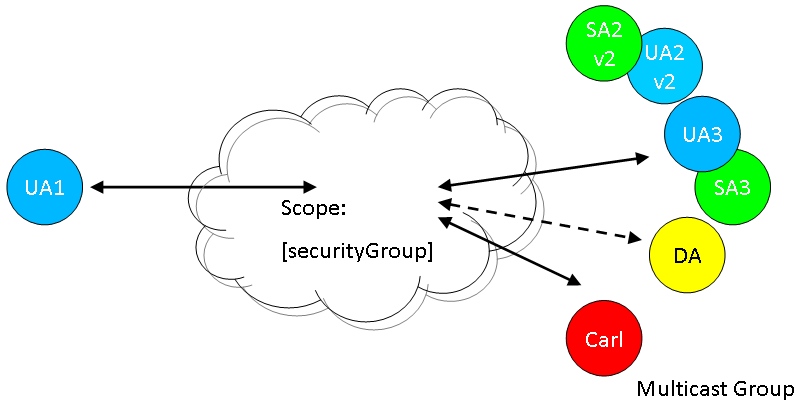
\includegraphics[width=0.5\textwidth]{Images/security-group_scope}
\caption{\label{fig:SecurityGroup-Scope}A dedicated scope denoting security groups. Since SG-advertisements are sent out using unencrypted SLPv2, attackers (Carl) are capable to discover SGs. However this does not pose a security threat.}
\end{figure}\noindent
Introducing SGs poses a chicken and egg problem on SecureSLP. How does a peer learn of the existence of a SG? Fortunately the functionality provided by traditional SLPv2 can be leveraged to advertise SGs via unencrypted service advertisements. However this allows an attacker to discover all available SGs. While the attacker will not be able to join the SG, it is essential that the advertisement does not leak confidential information as part of the service description. The only information which is essentially required is an SG identification that is best represented by public-key of the SG initiator.\\
Using a special service type that denotes a SG is one possibility how to make SGs discoverable by agents. This paper however takes a different approach and assigns a new keyword that marks a dedicated scope for SGs. This is favorable to a special service type since it practically hides SGs from legacy SLPv2 agents that would not be able to interact with a SG anyway (see \ref{sub:Protocols-basics}). Figure \ref{fig:SecurityGroup-Scope} depicts SG advertisement. The right side shows agents which are part of the same multicast group with the UA1 that queries for SGs. Agents marked with \emph{v2} ignore the query as it is not send to the default scope and are both not configured for the special scope explicitly.

\subsection{Security Groups and Directory Agents}
As stated earlier in this paper, DAs cause security implications for the security of SLP, which have to be accounted for. \citet{Hollick2001} does not address this topic and simply assumes the non-existence of DAs. This assumption is untenable in SLP as the fallback to DA mode is built into the protocol and UAs and SAs are required to use a DA if present (see \ref{sub:Protocols-basics}). Even though a forged DA would not be able to tamper with service descriptions due to integrity checks, it can prevent SGs from being established by silently discarding SG advertisements. Therefore SLP agents must revert to multicast convergence if a DA cannot be authenticated to be legit.\\
In case a DA is to be used together with SGs, it has to become a member of each and every group in the network. Otherwise it will not be able to decrypt the service description and answer queries sent by UAs.\\\\
The previous requirement and the ones listed in \ref{sub:Confidentiality-via-Security} make the Group Diffie-Hellman (GDH) outlined in \citet{Bhaskar2007} a good candidate as a GKA for SecureSLP.

%Chapter 4: Future Work
\section{Conclusion and Future Work}
Open networks become increasingly common due to the wide availability of mobile device technology. When such a device enters a network, it wants to learn about the services offered by other peers or advertise its own services. Service discovery protocols have been around to address this requirement for a while. A most prominent and widely adopted one is SLP. However, SLP has not been designed for open networks upfront. Thus the protocol has to undergo a renewal to make it fit for open networks.\\
This paper describes the fundamental security implications that arise from open networks. It picks up these implications in the scope of SLP and compiles a detailed threat analysis for SLP in open networks. It then continues to extend the current version of SLP with security enhancement to strengthen the protocol for use in untrustworthy and hostile environments by staying backward compatibility with earlier protocol versions. The major protocol modifications can be summarized as:
\begin{itemize}
\item SLPv2's pre-established trust model is replaced by a dynamic model that can deal with the dynamics of an open network. It is either implemented as a Public Key Infrastructure or a Web of Trust. On top a reputation based trust may be used when devices are not resource constrained by e.g. battery lifetime.
\item Confidentiality is added to SLP by encrypted group and peer to peer communication. The symmetric group key is handled by using Group Diffie-Hellman, a known protocol for distributed group key agreement. This goes beyond the approach taken by \citet{Hollick2001} who leaves confidentiality to the Internet layer. Thus our SecureSLP stays independent of additional network facilities.
\item SecureSLP is aware of all three agent types in SLP namely User Agents, Service Agents and Directory Agents. Where \citet{Hollick2001} excludes Directory Agents in his solution entirely, SecureSLP incorporates DAs into the protocol. This enables better performance and scalability when used in combination with the enhancements presented by \citet{Zhao2003}.
\end{itemize}
Table \ref{tab:SLP-and-SecureSLP} shows a comparison between traditional SLP and the secured version of SLP as proposed in this paper.
\begin{table}[!h]
\begin{centering}
\begin{tabular}{|c|c|c|}
\hline 
 & SLP & SecureSLP
\tabularnewline
\hline
\hline 
Authentication & $+$ & $+$
\tabularnewline
\hline 
Integrity & $+$ & $+$
\tabularnewline
\hline 
Confidentiality & $-$ & $+$
\tabularnewline
\hline 
Replay prevention & $-$ & $+$
\tabularnewline
\hline 
Authorization & $-$ & $\circ$
\tabularnewline
\hline 
Availability & $-$ & $-$
\tabularnewline
\hline 
Non-repudiation & $-$ & $-$
\tabularnewline
\hline
\end{tabular}
\par\end{centering}

\caption{\label{tab:SLP-and-SecureSLP}SLP and SecureSLP security comparision matrix}
\end{table}\\\\
With confidentiality being addressed in SecureSLP, peer authorization becomes feasible, to support different discovery results based on an UA authorization. Different authorization levels may be represented by a dedicated Security Group per level and Service Agent. However, more research has to be undertaken in order to validate this approach and add a concrete implementation to SecureSLP.\\
Properties like non-repudiation and availability are regarded as unessential for SecureSLP in the scope of this paper. Whether this assumption holds true and e.g. message loss and agent unavailability is indeed tolerated by the protocol, has to be confirmed in future work. Even more important is concise performance and scalability measurements to prove that the protocol extensions maintain SLP's performance characteristics even in large open networks with many peers and strong fluctuations.

%Chapter 5: Concepts for Implementation
\newpage
\section{Concepts for Implementation}
In chapters above we discussed some possible security concepts and increments for the service location protocol. In this section we will introduce our practical solutions to fulfill the requested requirements.\\
First of all we need to establish security groups, where users can communicate using encryption. To create those groups we combined the already implemented SLP scopes with a group key agreement protocol. For this purpose we took the Tree-based Group Diffie-Hellman protocol (TGDH). TGDH is a group key agreement protocol which we use to create and share security group keys (details about TGDH will be introduced in section \ref{sec:TGDH}). We will describe why we picked this protocol and how we integrated it into the SLP.\\
Further we will discuss possible attacks on SLP which uses TGDH and the solutions we made to prevent them. \textcolor{red}{(nachher etwas ausf�hrlicher beschreiben)}

\subsection{Security Groups}
Like discussed above we propose to create security groups in an open network to establish security between some users and still offer all SLP functions there. To create a secured group within an open network we worked out a concept and a new workflow for our SecuredSLP. First of all a security group in SecuredSLP is a SLP scope in which the group members use encryption to communicate with each other, which means the group members all share a secret. To create and share a secret we used the TGDH protocol. There are some requirements to a security group which we should look at:
\begin{itemize}
  \item To join a secured group a user needs to know that there is such a group and this information should be announced as a plain text message, otherwise it isn't possible to get knowlege about such a group. The message should contain at least the information about the group name and where to get access to this group.
  \item After a user is allowed to join a group, he requires the shared secret of this group, the group key (see also sections \ref{sec:TGDH} and \ref{sec:keyenchange}).
  \item With a valid group key the user can decrypt all announced service information or offer services itself.
  \item If a user leaves a secured group, reasons could be for example an expired session key, the secured group key should be refreshed automatically.
\end{itemize}
We choose TGDH because it fulfill all the requirements above and we already found an implementation in java for it. But it is not necessary to use TGDH, so any other group key agreement protocol would work as well.\\
With TGDH each user within a secured group has several cryptographic keys.\\
\textcolor{red}{�berarbeiten!!!}\\
\textbf{Group Shared Key (GSK):} This key is same for all group members and allows to access the secured group.\\
\textbf{Private-/Public-Key:} This is a key-pair that every user has and with those the users encrypt or decrypt their messages.

\subsection{Tree-based Group Diffie-Hellman (TGDH)}\label{sec:TGDH}
Tree-based Group Diffie-Hellman is a protocol-suite for group key management. It handles the key distribution between all network members. TGDH is based on a binary tree structure. But the tree structure is just logical and isn't connected with the real position of the network members. This protocol-suite handles several dynamic group events like a new member joins or leaves the group and two networks merge together or one network partitions in several networks. So TGDH implements four protocols: \textsl{join}, \textsl{leave}, \textsl{merge} and \textsl{partition}\footnote{To secure SLP we only use the join and leave protocols. For that reason the other protocols won't be discussed in detail.}. But all of these protocols have some common structures with following features:
\begin{itemize}
  \item Each network member computes the \textsl{group session key} out of the \textsl{group key} with a hash-function (the hash-function is the same for all members).
  \item Each \textsl{member session key} is just known to the member himself and shouldn't be published.
  \item In case a group gets larger, the \textsl{session keys} of new members will be included and some of old members have to refresh their \textsl{session key}.
  \item In case a group gets smaller, the \textsl{session keys} of the members, who left the group, will be deleted and at least one member of the group have to refresh his \textsl{session key}.
  \item All protocol-messages are signed by the sender. For the digital signature TGDH uses RSA or DSA with SHA-1 hash-function. 
\end{itemize}
After any changes each member refreshes his \textsl{key-tree} independently from each other.\\

\subsubsection{Keys in TGDH}
There are several cryptographic keys which are used in TGDH.
\begin{description}
\item[Group key] $K_{<0,0>}$ which is represented as the root of the TGDH tree (compare with figure \ref{fig:tgdh_tree}).
\item[Group session key] $K_{\text{\textit{group}}}$ which is derived from the group key. $K_{\text{\textit{group}}} = h(K_{<0,0>})$, where $h()$ is a cryptographic hash-function.
\item[Member session key] $K_i$ is a session key for the member $M_i$. 
\item[Blinded key] $BK_i$ is a key which can be calculated from the member session key $K_i$ with the function $BK_i = f(K_i)$, where $f() = g^k~mod~p$ with $g$ as generator and $p$ as a prime.
\end{description}
Furthermore there are also key sets a member has knowledge about. Each member knows all keys and their corresponding blinded keys in his path from the leaf to the root in the tree. For example member $M_2$ in the figure \ref{fig:tgdh_tree} knows the set of keys $\{K_{<2,1>}, K_{<1,0>}, K_{<0,0>}\}$ and the set of blinded keys $\{BK_{<2,1>}, BK_{<1,0>}, BK_{<0,0>}\}$. With that information it is possible to compute any other key:
\begin{align*}
K_{<l,v>} &= (BK_{<l+1, 2v+1>})^{K_{<l+1, 2v>}}~mod~p\\
&= (BK_{<l+1, 2v>})^{K_{<l+1, 2v+1>}}~mod~p\\
&= g^{K_{l+1, 2v}K_{l+1, 2v+1}}~mod~p\\
&= f(K_{l+1, 2v}K_{l+1, 2v+1})
\end{align*}
It is also possible to compute the group key out of that information. For member $M_2$ the calculation would be:
\begin{align*}
K_{<0,0>} &= (BK_{<1,1>})^{K_{<1,0>}}~mod~p\\
&= (BK_{1,1})^{(BK_{<2,1>})^{K_{<2,0>}}}~mod~p
\end{align*}
\begin{figure}[!h]
\centering
\includegraphics[width=0.5\textwidth]{Images/tgdh_tree}
\caption{Example of a tree structure in TGDH}
\label{fig:tgdh_tree}
\end{figure}

\subsubsection{Join protocol}
Assume a group with three members $\{M_1, M_2, M_3\}$ and a new member $M_4$ who wants to join this group. $M_4$ initialize the join protocol by sending a \textit{JoinMessage} to the group via multicast. The message contains the blinded key of $M_4$. First of all the join position for $M_4$ is calculated and a \textit{sponsor} is chose. The sponsor is the member whose leaf is placed on the insert position of the new member. In this case all members insert a new joint and a new leaf in their tree and delete all blinded keys in the path of the sponsor. Additionally the sponsor generates the new group session key and all keys and blinded keys in his path. Finally the sponsor sends the new tree $\widehat{T}$ and a set of all blinded keys via a multicast message. Member $M_1$ and $M_2$ can just calculate the group key after they received the new tree $\widehat{T}$. The tree update is shown in figure \ref{fig:tgdh_join}.
\begin{figure}[!h]
\centering
\includegraphics[width=0.5\textwidth]{Images/tgdh_join}
\caption{Tree update after a join of a new member}
\label{fig:tgdh_join}
\end{figure}

\subsubsection{Leave protocol}
To leave the group a member sends a \textit{LeaveMessage} via multicast to the group. Same as in join protocol, a sponsor is chose. All members remove the leaf and his father joint from the tree. Also they remove all keys and blinded keys in the corresponding path. Additionally the sponsor generates new session key and computes all keys and blinded keys in his path. In the end sponsor sends the new tree $\widehat{T}$ and a set of all blinded keys via broadcast to the group. After receiving the new tree, all other members are able to compute the new group key. The corresponding tree update is illustrated in figure \ref{fig:tgdh_leave}.
\begin{figure}[!h]
\centering
\includegraphics[width=0.5\textwidth]{Images/tgdh_leave}
\caption{Tree update after a member left the group}
\label{fig:tgdh_leave}
\end{figure}

%Chapter 6: Integration of a group key agreement protocol into SLP
\section{Integration of a group key agreement protocol into SLP}
There are two main approaches how to integrate a group key agreement protocol into the SLP. It is possible to integrate the group key agreement hardcoded into SLP or as a module adjacent to SLP. Both have benefits and disadvantages. 

\subsection{Hardcoded integration}
With this solution we have to take the SLP specification apart and change many methods to combine a group key agreement protocol with SLP. Such integration means that we need not just some changes but a very new communication workflow with new message formats and timeout behavior. Furthermore the group key agreement protocol couldn't be replaces anymore so all users would be bind to a special group key agreement protocol. That could be a neatly solution but would change the SLP too much and the implementation would be much complicated. Also the SLP wouldn't be compatible to the versions below and that isn't our goal. This approach would deliver a new protocol which probably would scale better as the modular integration solution.

\subsection{Modular integration}
With this solution we don't make many changes in the SLP specification. We use a group key agreement protocol as a module which we combine with SLP without fully integrates it into the SLP specification. In this way the module can easily be replaced anytime. So we are not bound to a special group key agreement protocol. Also it is possible to use many several group agreement protocols at the same time if needed. Our goal was to upgrade the SLP with minimum changes but to solve the requested requirements like discussed in section \ref{sec:conclusion}, so we decided to take this solution. Furthermore this solution can be applied much easier on current SLP implementation as a hardcoded integration.\\
For this purpose we have minor changes in the source code. Like discussed above we took TGDH as our group agreement protocol. To make SLP work with TGDH we had to change the header of SLP messages and implement additional functions into SLP to communicate with our group agreement protocol. A disadvantage of this method is a bigger communication overhead because SLP and the group key agreement protocol don't work synchronized together.

\subsubsection{Workflow of SLP with a modular integration}
\textcolor{red}{hier noch ein Bild einf�gen}

%Chapter 7: Implementation
\section{Implementation}
To combine SLP with our group key agreement protocol we changed/added following protocol properties:
\begin{itemize}
  \item SLP message
  \item Key enchantment
  \item Communication
\end{itemize}

\subsection{SecuredSLP message format}
The header of a SLP message was modified to distinguish SLP messages from SecuredSLP messages. We added the \texttt{S}, \texttt{Security Group Length} and \texttt{Security Group Name} flags into the header and changed the \texttt{Version} of SLP in the source code (compare figure \ref{fig:slp-header} and figure \ref{fig:sslp-header}).
\begin{description}
\item[Version:] Is now set to 3.
\item[S:] This flag shows that the message body is encrypted.
\item[Security Group Length:] This flag specifies the length of the \texttt{Security Group Name} string.  
\item[Securety Group Name:] This flag shows the name of the security group the message belongs to.
\end{description}

\begin{figure}[!h]
\begin{lstlisting}
	 0                   1                   2                   3
	 0 1 2 3 4 5 6 7 8 9 0 1 2 3 4 5 6 7 8 9 0 1 2 3 4 5 6 7 8 9 0 1
	+-+-+-+-+-+-+-+-+-+-+-+-+-+-+-+-+-+-+-+-+-+-+-+-+-+-+-+-+-+-+-+-+
	|    Version    |  Function-ID  |            Length             |
	+-+-+-+-+-+-+-+-+-+-+-+-+-+-+-+-+-+-+-+-+-+-+-+-+-+-+-+-+-+-+-+-+
	| Length, contd.|O|F|R|       reserved          |Next Ext Offset|
	+-+-+-+-+-+-+-+-+-+-+-+-+-+-+-+-+-+-+-+-+-+-+-+-+-+-+-+-+-+-+-+-+
	| Next Extension Offset, contd. |              XID              |
	+-+-+-+-+-+-+-+-+-+-+-+-+-+-+-+-+-+-+-+-+-+-+-+-+-+-+-+-+-+-+-+-+
	|      Language Tag Length      |         Language Tag          |
	+-+-+-+-+-+-+-+-+-+-+-+-+-+-+-+-+-+-+-+-+-+-+-+-+-+-+-+-+-+-+-+-+
\end{lstlisting}
\label{fig:slp-header}
\caption{SLPv2 Header}
\end{figure}

\begin{figure}[!h]
\begin{lstlisting}
	 0                   1                   2                   3
	 0 1 2 3 4 5 6 7 8 9 0 1 2 3 4 5 6 7 8 9 0 1 2 3 4 5 6 7 8 9 0 1
	+-+-+-+-+-+-+-+-+-+-+-+-+-+-+-+-+-+-+-+-+-+-+-+-+-+-+-+-+-+-+-+-+
	|    Version    |  Function-ID  |            Length             |
	+-+-+-+-+-+-+-+-+-+-+-+-+-+-+-+-+-+-+-+-+-+-+-+-+-+-+-+-+-+-+-+-+
	| Length, contd.|O|F|R|S|     reserved          |Next Ext Offset|
	+-+-+-+-+-+-+-+-+-+-+-+-+-+-+-+-+-+-+-+-+-+-+-+-+-+-+-+-+-+-+-+-+
	| Next Extension Offset, contd. |              XID              |
	+-+-+-+-+-+-+-+-+-+-+-+-+-+-+-+-+-+-+-+-+-+-+-+-+-+-+-+-+-+-+-+-+
	|      Language Tag Length      |         Language Tag          |
	+-+-+-+-+-+-+-+-+-+-+-+-+-+-+-+-+-+-+-+-+-+-+-+-+-+-+-+-+-+-+-+-+
	|      Security Group Length    |      Security Group Name      |
	+-+-+-+-+-+-+-+-+-+-+-+-+-+-+-+-+-+-+-+-+-+-+-+-+-+-+-+-+-+-+-+-+
\end{lstlisting}
\label{fig:sslp-header}
\caption{SecuredSLP Header}
\end{figure}
Additionally we use a HMAC (96 Bit) over the header and add it into the encrypted message body so the header and payload are linked with each other. This method is also used in IPSec under the ESP mode and allows us to prevent replay attacks and header manipulation of each SecuredSLP message. See also \textcolor{red}{quellen nachher einf�gen}

\subsection{Key enchantment in SecuredSLP}\label{sec:keyenchange}
Like discussed above we use a group key agreement protocol to establish security between group members. To get knowledge about a security group, clients use extra discovery iteration. The information about a security group is announced as plain text; otherwise no one would be able to join such a group. To join a security group a user has to send a join message to the group. Then the group key agreement protocol handles the key distribution. In our implementation we used TGDH, so the distribution works like discussed in section \ref{sec:TGDH}. After receiving the group key, security group members are able to discover services which are pronounced in this security group or provide services themselves. Also there is a rekeying phase after a user leaves the group. That is important to keep the security under the group members and to avoid that a key gets compromised.

\subsection{Communication in SecuredSLP}
Due to the additional changes in the protocol it is necessary to take a look at the communication between network members. SecuredSLP still provides unencrypted communication like in SLPv2 so it is still possible to create or join a unsafe SLP scope. In that case the communication works like in SLPv2 (compare section \ref{sec:intro}) without a group agreement protocol. In case SecuredSLP tries to establish connection to a security group the communication can be described as following:
\begin{enumerate}
  \item User discovers a security group and sends a \textit{JoinMessage} to the group key agreement protocol (TGDH in our case)
  \item Group key agreement protocol initializes the rekeying phase for the security group and computes new group key.
  \item New member receives the group key and is able to communicate with the other security group members. Compare with figure \ref{fig:sslp_join}
\end{enumerate}
\begin{figure}[!h]
\centering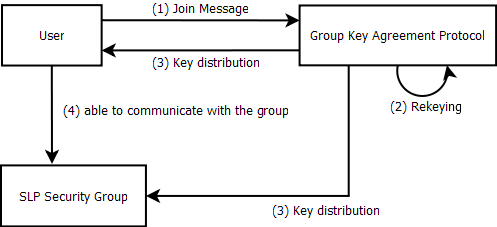
\includegraphics[width=0.5\textwidth]{Images/sSLP_join}
\label{fig:sslp_join}
\caption{Communication sequence of a user joining a SecuredSLP security group}
\end{figure}
Like told above the group agreement protocol is just a module adjacent to SLP and works asynchronous with it. Hence the key distribution is more complicated and fault-prone. Also there is just one valid key in the network at time so most problems arrive if a rekeying phase is initialize and there are still messages in the network encrypted with the old group key. Those messages will be refused by SecuredSLP.

%Chapter 8: Possible Attacks on SecuredSLP
\section{Possible attacks on SecuredSLP}
In this section we want to discuss which general attacks are possible on SecuredSLP and how they are prevented or why they can't be prevented.

\subsection{Denial of Service (DoS) attacks}\label{sec:DoS}
Like all distributed systems SecuredSLP suffers from DoS attacks. In SecuredSLP there are two attacking points for a DoS attack. The first one is to overfeed the UA/SA/DA with information or requests. In this scenario an attacker requests for example information about a service from a DA and prevents the usage of that DA by other network members. The second attacking point appears just if the secure mode of SecuredSLP is enabled and a group key agreement protocol is used. In that case an attacker could initiate join/leave messages so the network would stuck in the rekeying phase. This problem is especially present in the group key agreement protocols which provide forward and backward security like in the case of TGDH. Each time a user joins or leaves the network the TGDH initiates a rekeying phase so an attacker could exploit this feature.\\
There is no neat way to prevent attacks on UA/SA/DA because that's their purpose to send or answer requests. It would be possible to drop messages from a user who sends too many requests but this is not part of our paper so it won't be discussed here in detail. To prevent or reduce DoS attacks on the group key agreement protocol it is possible to use another protocol as TGDH. The keys could also be distributed by a centralized infrastructure like a key distribution center (KDC) or even a network administrator so there wouldn't be rekeying phase all the time. If we set special intervals for the rekeying phase, we automatically assume that the security group can't be compromised in such an interval. This solution lowers the security of a group because it gives an opportunity for an attacker to use a compromised key in an interval. Such a distribution could just work in a closed network with stable security groups but not for our case in open networks.

\subsection{Replay attacks}
In SecuredSLP a possibility of a replay attacks is very low. To prevent replay attacks we made sure that the header of each message can't be manipulated. Therefore we make a HMAC over the message header and include it into the message which is encrypted.  A SecuredSLP message contains a \texttt{XID} which marks the message and binds it to a sequence of messages (compare with figure \ref{fig:sslp-header}) and the payload is encrypted and signed by the sender. That prevents that an attacker can change the header information without the receptor getting knowledge about. The only replay attack would be to use a current message to overfeed a peer with it which could count as a DoS attack (see section \ref{sec:DoS}).

\subsection{Evedrop attacks}
Evedrop attacks are still possible on the SecuredSLP. Everyone can log the network traffic and learn about its behavior. The benefit in SecuredSLP is that the information stays confidentiality because all messages are encrypted and signed. An attacker can just intercept messages and read the message header but not decrypt the payload as we assume that the encryption algorithms are safe.

\subsection{Manipulation attacks}
Like told above we exclude the manipulation of SecuredSLP messaged because the messages are encrypted and signed and the header of each message is linked with the payload using HMAC. For more information about HMAC see \cite{Kraw97} and \cite{Kero00}.

\subsection{Man-in-the-middle attacks}
Man-in-the-middle attacks still work on SecuredSLP. For example an attacker can act as a DA in a security group and communicate with his prey and get information about the services he provides or use. \textcolor{red}{muss wahrscheinlich raus!}

%Chapter 9: evaluation
\section{Evaluation}\label{sec:evaluation}
The integration and implementation of the suggested solutions were successful.
The specifications of common SLP were extended for confidentiality, integrity,
authentication and replay attack prevention. The result of this extension is
the SecuredSLP specification and it provides fundamental security features
which are needed for a secure communication in an open network. Current
SecuredSLP is implemented as a ``proof of concept'' version and works with TGDH
as its group key agreement protocol. But the SecuredSLP specification is not
bound to a special protocol, any other group key agreement protocol could be
integrated instead. It is also possible to add or change the cipher-suite and
use other cryptographic algorithms. In current state the implementation is
limited to RSA.\\\\ But there are not only positive aspects resulting from the
extension to SecuredSLP. Several problems occur by useging different
group key agreement protocols. First of all the secured groups demand extra
discovery iteration. In the first discovery iteration a user is only able to
discover all plain scopes. To discover the security scopes/groups the user
needs a second discovery iteration. That means that the time to discover a
security group is doubled and this is process deterioration especially in an
open network with low performance devices. Another problem is the group key
agreement protocol with forward/backward secrecy features. The rekeying phase of
the group key agreement protocol always disturbs the workflow of the service
location protocol. A short time after rekeying old keys are useless and won't
be accepted for the communication. So if the network is unstable and dynamic
the rekeying phase becomes a thread. If many users join/leave the security
group the security group will be stuck in the rekeying phase (compare section
\ref{sec:DoS}). For that purpose we get validation intervals for the group
shared keys. That means we dynamically keep several old group shared keys
valid. The number of the keys, which are valid at a time, depends on the
network behavior and changes on demand. We reduce the number of keys valid at a
time. In that way we minimize the intervals where the security group members
are not able to communicate but we still keep the security of the group shared
key(s) high. This feature is already implemented in the current SecuredSLP
version but not tested. The right balance for that algorithm is not set yet.
Also the scale ability of SecuredSLP with a large number of users in a security
group has not been tested practically yet. But we assume that it will work
with several hundred users. We did not apply any trust model to the SecuredSLP
implementation. That means anyone, who wants to join a security group, can get
the access.\\ \hrule The extension from common SLP to SecuredSLP is a first
step to increase the security of the service location protocol especially for
the use in a new environment like an open network. SLP was not originally
designed for the usage in open networks. In the first and second sections of
this paper we introduce the workflow of a service discovery protocol itself and
its issues and the problems while using it in an open network. In section
\ref{sec:slp-overview} some useful solutions are presented and discussed how to
raise the security of this protocol. An overview of the suggested solutions can
be found in section \ref{sec:conclusion}. In sections 5 - 9 the introduced
solutions were applied to the SLP specification and a ``proof of concept''
version of SecuredSLP was implemented. Those sections describe how and why the
integration of security has been done.


%References
\bibliographystyle{plainnat}
\clearpage\addcontentsline{toc}{chapter}{\bibname}
\bibliography{Kapitel/references}
\end{document}